\documentclass[11pt]{article}  

%%%%%%%% PREÁMBULO %%%%%%%%%%%%
\title{Portada reporte practicas}

\usepackage{tikz}
\usetikzlibrary{positioning, arrows.meta}
\usetikzlibrary{shapes.geometric, arrows}
\usetikzlibrary{positioning, arrows.meta}
\usetikzlibrary{positioning, arrows.meta}
\usepackage[spanish]{babel} 
\usepackage[utf8]{inputenc}    
\usepackage{amsmath} 
\usepackage{xcolor}

%\usepackage{amssymb} 
\usepackage{graphicx} 
\usepackage{color} 
\usepackage{subfigure} 
\usepackage{float} 
\usepackage{capt-of} 
\usepackage{sidecap} 
	\sidecaptionvpos{figure}{c} 
\usepackage{caption} 
\usepackage{commath}  

\usepackage{cancel} 
 
\usepackage{anysize} 					
\marginsize{2cm}{2cm}{2cm}{2cm} 

\usepackage{appendix}
\renewcommand{\appendixname}{Apéndices}
\renewcommand{\appendixtocname}{Apéndices}
\renewcommand{\appendixpagename}{Apéndices} 

\usepackage[colorlinks=true,plainpages=true,citecolor=blue,linkcolor=blue]{hyperref}

\usepackage{fancyhdr} 
\pagestyle{fancy}
\fancyhf{}
\fancyhead[L]{\footnotesize UPIITA} 
\fancyhead[R]{\footnotesize IPN}   
\fancyfoot[R]{\footnotesize Programacion Avanzada}  
\fancyfoot[C]{\thepage} 
\fancyfoot[L]{\footnotesize Ing. Mecatrónica}  
\renewcommand{\footrulewidth}{0.4pt}


\usepackage{listings} 
\definecolor{dkgreen}{rgb}{0,0.6,0} 
\definecolor{gray}{rgb}{0.5,0.5,0.5}

\tikzstyle{startstop} = [rectangle, rounded corners, minimum width=3cm, minimum height=1cm,text centered, draw=black, fill=red!30]
\tikzstyle{process} = [rectangle, minimum width=3cm, minimum height=1cm, text centered, draw=black, fill=orange!30]
\tikzstyle{io} = [trapezium, trapezium left angle=70, trapezium right angle=110, minimum width=3cm, minimum height=1cm, text centered, draw=black, fill=blue!30]
\tikzstyle{decision} = [diamond, minimum width=3cm, minimum height=1cm, text centered, draw=black, fill=green!30]
\tikzstyle{arrow} = [thick,->,>=stealth] 

% configuración para el lenguaje que queramos utilizar
\lstnewenvironment{python}[1][]
{
    \lstset{
        language=Python,
        basicstyle=\small\ttfamily,
        keywordstyle=\color{blue}\bfseries,
        commentstyle=\color{green!60!black},
        stringstyle=\color{red},
        showstringspaces=false,
        frame=single,
        numbers=left,
        numberstyle=\tiny,
        numbersep=5pt,
        #1
    }
}
{}
\title{Plantilla portada}

%%%%%%%% TERMINA PREÁMBULO %%%%%%%%%%%%

\begin{document}

%%%%%%%%%%%%%%%%%%%%%%%%%%%%%%%%%% PORTADA %%%%%%%%%%%%%%%%%%%%%%%%%%%%%%%%%%%%%%%%%%%%
																					%%%
\begin{center}																		%%%
\newcommand{\HRule}{\rule{\linewidth}{0.5mm}}									%%%\left
 																					%%%
 																					
\begin{minipage}{0.48\textwidth} \begin{flushleft}

\includegraphics[scale = 0.63]{logo_upiita.png}
\end{flushleft}\end{minipage}
\begin{minipage}{0.48\textwidth} \begin{flushright}

\includegraphics[scale = 0.35]{IPN.jpg}
\end{flushright}\end{minipage}

													 								%%%
\vspace*{-1.5cm}								%%%
																					%%%	
\textsc{\huge Instituto Polit\'ecnico\\ \vspace{5px} Nacional}\\[1.5cm]	

\textsc{\LARGE Unidad Profesional Interdisciplinaria en Ingenier\'ia y				%%%
Tecnolog\'ias Avanzadas}\\[1.5cm]													%%%

\begin{minipage}{0.9\textwidth} 
\begin{center}																					%%%
\textsc{\LARGE Programación Avanzada 2MV7}
\end{center}
\end{minipage}\\[0.5cm]
%%%
    																				%%%
 			\vspace*{1cm}																		%%%
																					%%%
\HRule \\[0.4cm]																	%%%
{ \huge \bfseries Practica 4}\\[0.4cm]	%%%
 																					%%%
\HRule \\[1.5cm]																	%%%
 																				%%%
																					%%%
\begin{minipage}{0.46\textwidth}													%%%
\begin{flushleft} \large															%%%
\emph{Autor:}\\	
Barrios Mendez Jose Alberto\\
Boleta: 2022640111


%%%
			%\vspace*{2cm}	
            													%%%
										 						%%%
\end{flushleft}																		%%%
\end{minipage}		
																%%%
\begin{minipage}{0.52\textwidth}		
\vspace{-0.6cm}											%%%
\begin{flushright} \large															%%%
\emph{Profesor:} \\																	%%%
Cruz Mora Jose Luis\\
													%%%
\end{flushright}																	%%%
\end{minipage}	
\vspace*{1cm}
%\begin{flushleft}
 	
%\end{flushleft}
%%%
 		\flushleft{\textbf{\Large Ing. Mecatrónica}	}\\																		%%%
\vspace{2cm} 																				
\begin{center}																					
{\large \today}																	%%%
 			\end{center}												  						
\end{center}							 											
																					
\newpage																		
%%%%%%%%%%%%%%%%%%%% TERMINA PORTADA %%%%%%%%%%%%%%%%%%%%%%%%%%%%%%%%

\tableofcontents 

\newpage

\section{Objetivo.}

Crear aplicaciones con diferentes graficas de usuarii (GUI) utilizando controles basicos

\section{Introduccion.} 
En esta presente practica, continuaremos con el aprendizaje de  python, de forma mas espefica abordaremos las interfaces graficas, con ayuda de las librerias Pyqt6 y su diseñador  de interfaces  graficas, nos va a facilitar el crear la interfaz grafica, ya que de otra forma tendriamos que programar cada boton y que este corresponda dentro del lugar deseado. Con la ayuda de pyqt6,daremos solucion al programa que se plantea, el cual es diseñar una calculadora con las operaciones basicas. En este reporte abordaremos la forma en darle solucion con la libreria anteriormente mencionada 



\section{Desarrollo.}


\subsection{Creacion de la interfaz}
Con ayuda del "Qt Disigner", el cual esta incluido dentro de las herramientas o "tools" de pyqt6, podemos  abrir una GUI, la cual nos brinda una pantalla con varias opciones, para empezar a DISEÑAR nuestra calculadora, es importante recalcar que en este paso unicamente nos vamos a centrar en el diseño de la interfaz, la implementacion de las opciones que se muestran o la configuracion de los botones se realiza posteriormente. 


\begin{figure}[H]
		\begin{center}
 			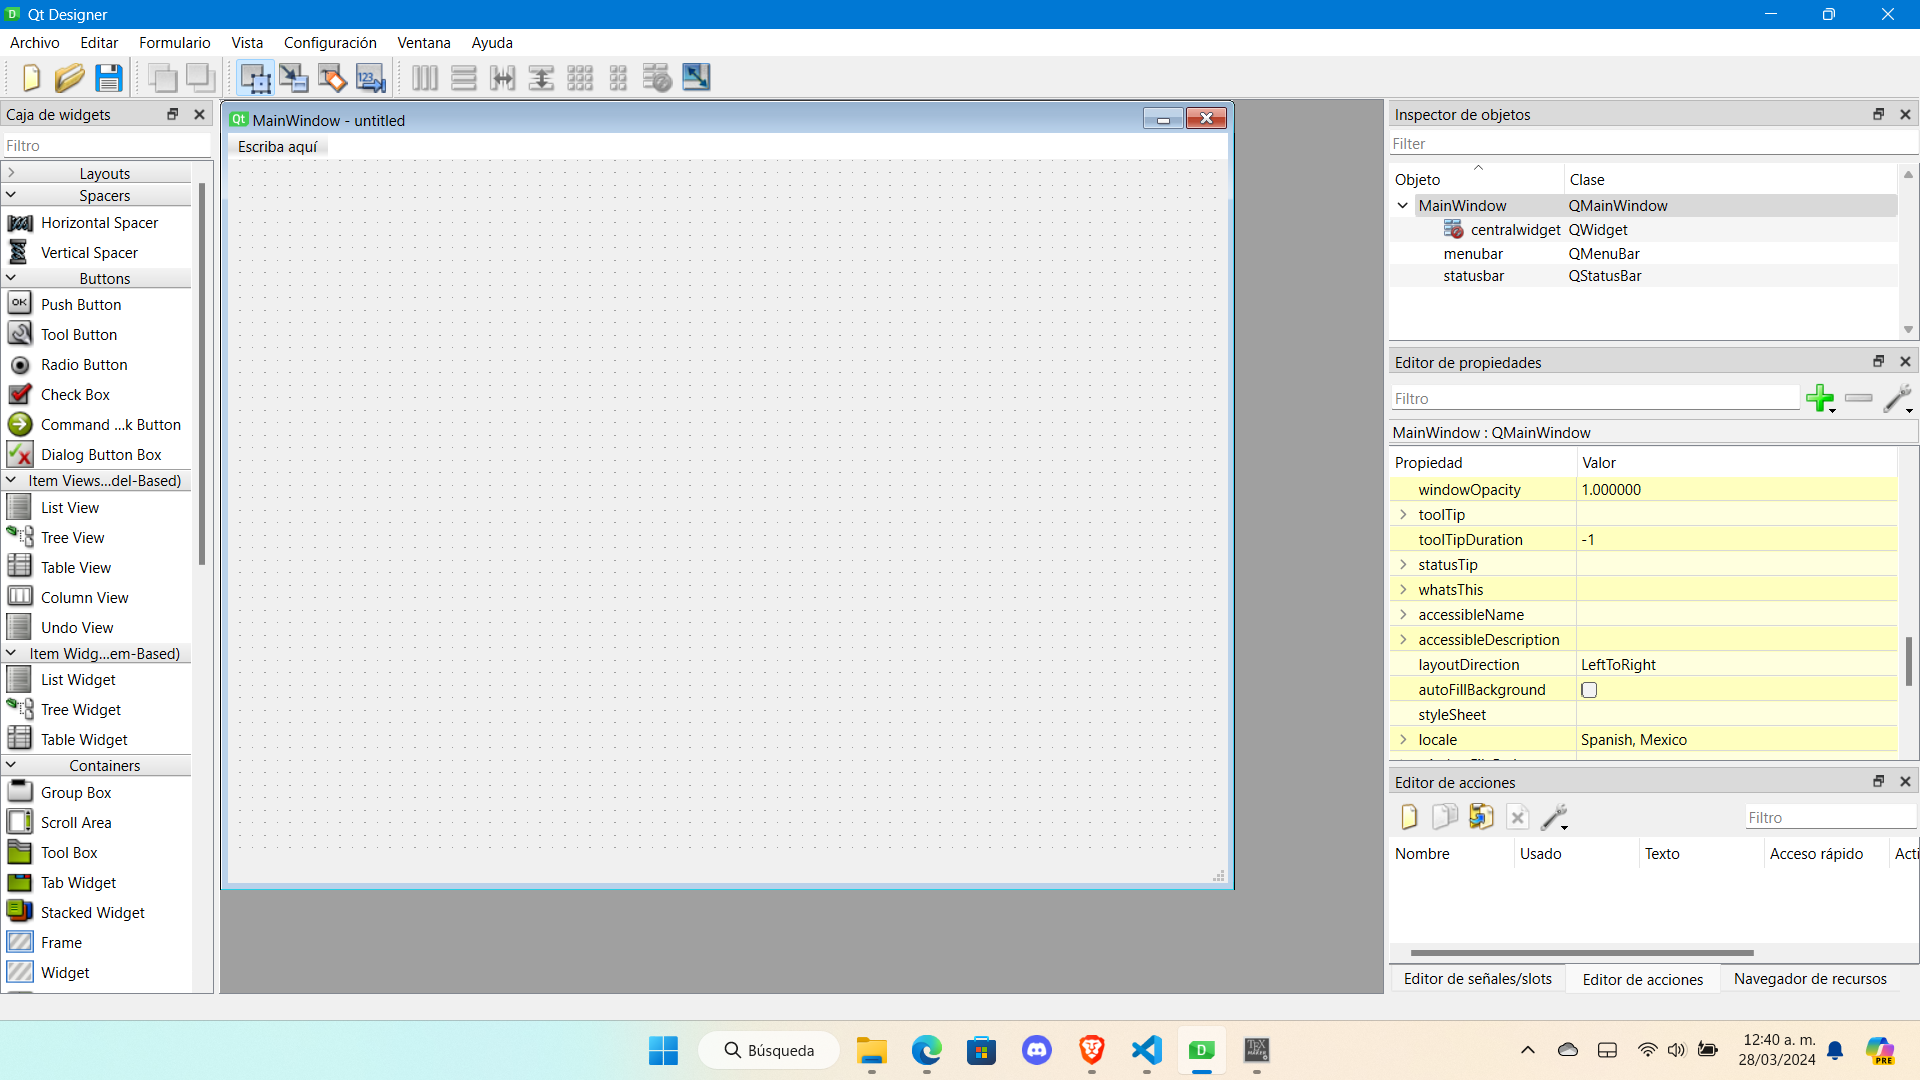
\includegraphics[width = .8\textwidth]{01.png}
 			\captionof{figure}{\label{fig:IPN}Interfaz de Qt Designer} 
 			
		\end{center} 
\end{figure}

Aqui vamos a empezar por el diseño de nuestra calculadora, para ello vamos utilizar 2 tipos de herramientas.
\begin{enumerate}
\item PushButtom: Esto nos va a servir como un boton de toda la vida, al presionarlo realizara alguna accion, en nuestro caso solo agregara numero o calculara las operaciones.
\item QLabel: Esto nos va a servir para poder mostrar los numeros que queremos cuando presionemos algun, numero o seleccionemos alguna operacion, es decir la funcionalidad es mostrar el texto en un recuadro
\end{enumerate}

Una vez definios los tipos de herramientas a usar, continuaremos con el diseño de la calculadora para esto, yo elegi el siguiente diseño.

\begin{figure}[H]
		\begin{center}
 			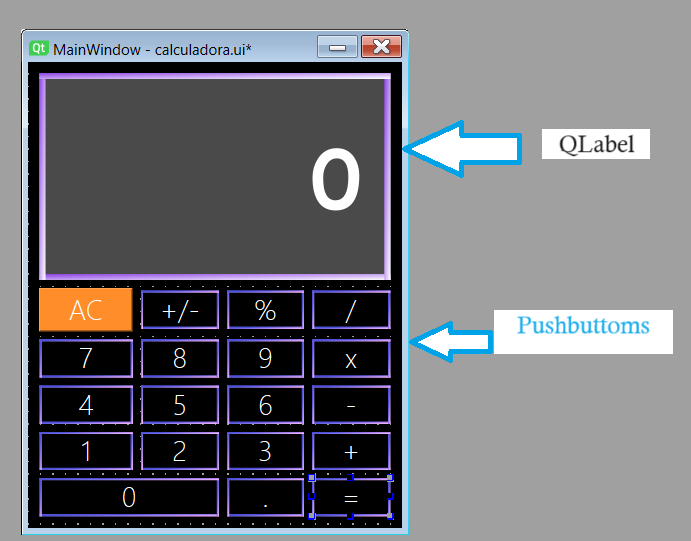
\includegraphics[width = .6\textwidth]{02.png}
 			\captionof{figure}{\label{fig:IPN}Diseño de la interfaz para la calculadora} 
 			
		\end{center} 
\end{figure}

\subsection{Compilacion}
Una vez realizado este paso, procedemos a guardar nuestro archivo, el cual se guarda con la extension .ui, para poder ejecutarlo como archivo python, es necesario realizar lo siguiente. Primero debemos usar una plantolla, la cual es vista en clase, con esta plantilla conseguiremos heredar el archivo .ui, todas las caracteristicas y atributos, pero con la diferencia que ahora le podremos agregar el backend, necesario para lograr que nuestra calculadora funcione de manera correcta.
Antes de empezar a programar las funciones, es necesario crear un segundo archivo con extension python, esto es por lo siguiente.\\
Cuando nosotros obtenemos el primer archivo .py, este contiene toda la interfaz, es decir, es como si hubieramos diseñado la interfaz en este archivo, por lo cual es un archivo poco practico para implementar todo el backend, de tal forma que los archivos nos quedaran de la siguiente forma.
\begin{figure}[H]
		\begin{center}
 			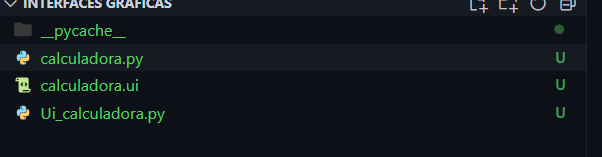
\includegraphics[width = .6\textwidth]{03.png}
 			\captionof{figure}{\label{fig:IPN}Archivos } 
 			
		\end{center} 
\end{figure}

\subsection{Implementacion de cada funcion}
Para esta parte, viene lo realmente complejo, ya que aqui es donde va a ocurrir la magia, en esta parte debemos definir que es lo que va a realizar cada boton, para esto, se implemento de la siguiente forma. Dentro de la clase principal "MainWindow" vamos a declarar el constructor, el cual contenera lo siguiente. 

\begin{figure}[H]
		\begin{center}
 			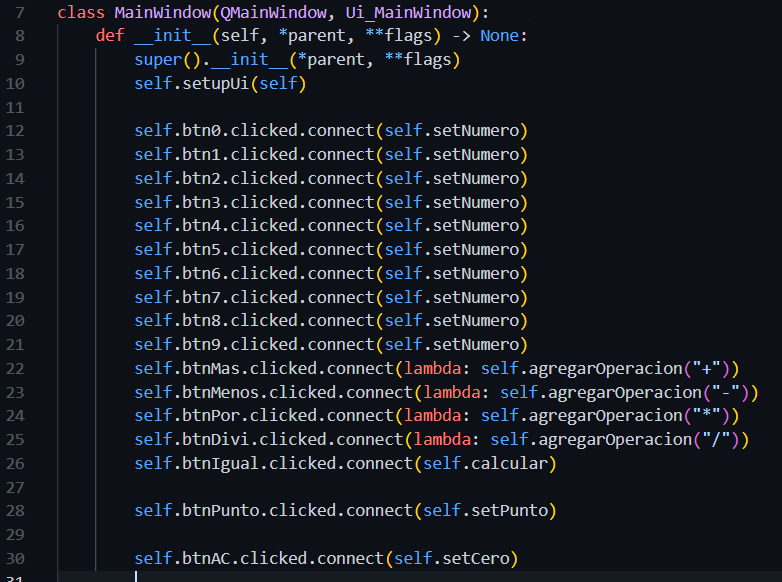
\includegraphics[width = .6\textwidth]{04.png}
 			\captionof{figure}{\label{fig:IPN}Constructor de la clase principal} 
 			
		\end{center} 
\end{figure}
Lo que hace es conectar las señales (eventos) emitidas por los botones de la interfaz gráfica con las funciones correspondientes que manejan las acciones del usuario.\\
'self.btn0.clicked.connect(self.setNumero)' Conecta la señal "clicked" del botón "btn0" con la función "setNumero", lo que significa que cuando se haga clic en el botón "btn0", se llamará a la función "setNumero". Lo mismo ocurre para los botones btn1 a btn9, que están conectados a la función setNumero. Esto significa que cuando cualquiera de estos botones numéricos es presionado, se agrega el número correspondiente a la pantalla de la calculadora.\\
self.btnMas.clicked.connect(lambda: self.agregarOperacion("+")): Conecta la señal clicked del botón btnMas con una función lambda que llama a agregarOperacion con el argumento +. Esto significa que cuando se haga clic en el botón btnMas, se llamará a agregarOperacion con el operador +. Lo mismo ocurre para los botones de operación btnMenos, btnPor y btnDivi, que están conectados a funciones lambda que llaman a agregarOperacion con los operadores -, * y /.
self.btnIgual.clicked.connect(self.calcular): Conecta la señal clicked del botón btnIgual con la función calcular

\begin{figure}[H]
		\begin{center}
 			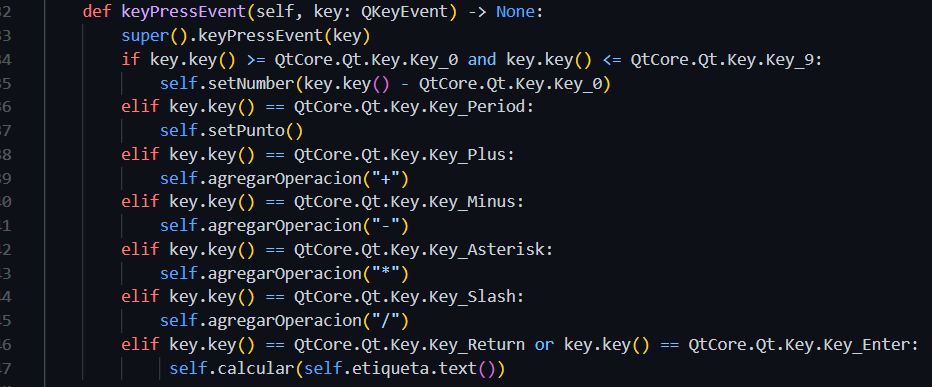
\includegraphics[width = .6\textwidth]{05.png}
 			\captionof{figure}{\label{fig:IPN}Metodo para manejar los eventos del teclado } 
 			
		\end{center} 
\end{figure}

Este método keyPressEvent es responsable de manejar los eventos de teclado en la ventana de la calculadora

El metodo verifica que tecla es la que fue presionada y realiza la accion correspondiente:\\
\begin{itemize}
\item Si la tecla presionada es un número (0 a 9), llama a la función self.setNumber() con el número correspondiente.
\item Si la tecla presionada es el punto (.), llama a la función self.setPunto() para agregar un punto decimal.
\item Si la tecla presionada es la tecla de suma (+), resta (-), multiplicación (*) o división (/), llama a la función self.agregarOperacion() con el operador correspondiente.
\item Si la tecla presionada es la tecla de enter , llama a la función self.calcular() con la expresión actual en la etiqueta de la calculadora 
\end{itemize}

Ahora pasemos con los siguiente metodos

\begin{figure}[H]
		\begin{center}
 			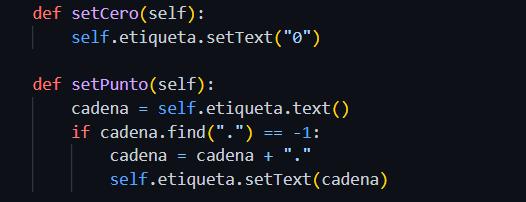
\includegraphics[width = .6\textwidth]{06.png}
 			\captionof{figure}{\label{fig:IPN}Metodos para poner 0 y para poner punto} 
 			
		\end{center} 
\end{figure}

Estos metodos son triviales ya que hacen lo siguiente:
\begin{itemize}
\item SetCero: Unicamente borra los datos ingresados, o visto de otra forma, vuelve al estado inicial de la calculadora.
\item SetPunto: metodo para agregar el punto decimal a un numero ingresado, verifica que no se agregue mas de uno, con el fin de que el codigo funcione correctamente
\end{itemize}

\begin{figure}[H]
		\begin{center}
 			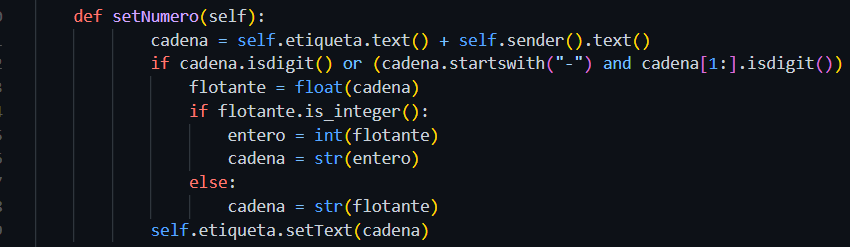
\includegraphics[width = .6\textwidth]{07.png}
 			\captionof{figure}{\label{fig:IPN}Metodo para agregar digitos al QLabel} 
 			
		\end{center} 
\end{figure}

Este método, llamado setNumero, esta diseñado para manejar el evento de click, en cualquier boton de la interfaz
\begin{itemize}
\item  cadena = self.etiqueta.text() + self.sender().text() obtiene el texto actual de la etiqueta de la calculadora y lo concatena
 Luego, se verifica si la cadena resultante después de la concatenación cumple con alguna de las siguientes condiciones:

\item Es una cadena de dígitos (números enteros).
\item Comienza con un signo menos (-) y el resto de la cadena son dígitos (números enteros).
\item Contiene un punto (.) y el resto de la cadena son dígitos o puntos (números en formato de punto flotante).
Si alguna de estas condiciones se cumple, se convierte la cadena a un número en formato de punto flotante (float(cadena)). Luego se verifica si el número es un enter (flotante.isinteger()). Si es un entero, se convierte a entero y se convierte nuevamente a cadena (str(entero)). Si no es un entero, se deja como está.

\item Finalmente, se establece el texto de la etiqueta de la calculadora con la cadena resultante
\end{itemize}

Ahora vamos a revisar el metodo para calcular las operaciones.
\begin{figure}[H]
		\begin{center}
 			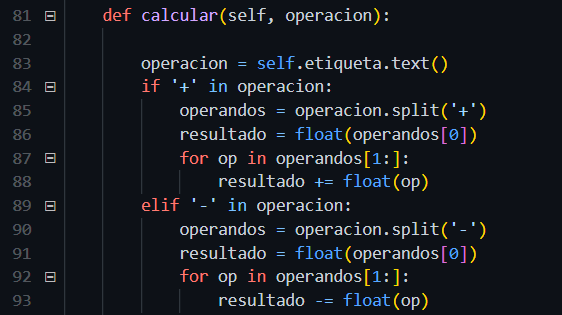
\includegraphics[width = .6\textwidth]{08.png}
 			\captionof{figure}{\label{fig:IPN}Metodo para calcular las operaciones} 
 			
		\end{center} 
\end{figure}
  Este método se encarga de realizar la evaluación de la expresión matemática presente en la etiqueta de la calculadora y mostrar el resultado en la misma etiqueta.
\begin{itemize}
    
    \item \textbf{Pasos:}
    \begin{enumerate}
        \item Se obtiene la expresión matemática actualmente mostrada en la etiqueta de la calculadora mediante la asignación \( \text{operacion} = \text{self.etiqueta.text()} \).
        \item Se verifica qué operador está presente en la expresión (\(+\), \(-\), \(*\), \(/ \)) utilizando condicionales \texttt{if}, \texttt{elif} y \texttt{else}.
        \item Dependiendo del operador encontrado, se divide la expresión en una lista de operandos mediante el método \texttt{split()}. Por ejemplo, si la expresión es "5+3", se dividirá en \(["5", "3"]\).
        \item Se inicializa la variable \texttt{resultado} con el primer operando convertido a un número de punto flotante mediante la expresión \texttt{float(operandos[0])}.
        \item Se itera sobre los operandos restantes y se realiza la operación correspondiente con cada uno de ellos.
        \item Si la operación implica una división y el divisor es cero, se establece el resultado como "Error". De lo contrario, se realiza la división normalmente.
        \item Finalmente, se establece el resultado calculado como el texto de la etiqueta de la calculadora mediante la expresión \texttt{self.etiqueta.setText(str(resultado))}.
    \end{enumerate}
\end{itemize} 

\section{Resultados.}


\begin{figure}[htbp]
  \begin{minipage}[b]{0.5\textwidth}
    \centering
    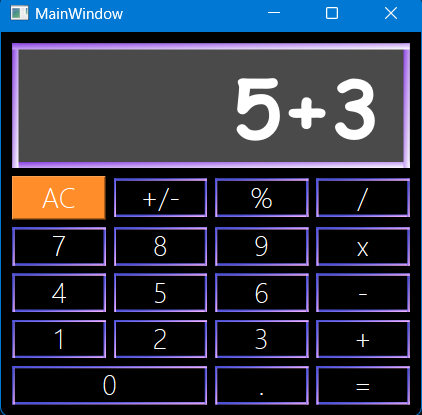
\includegraphics[width=\textwidth]{09.png}
    \caption{}
    \label{fig:imagen1}
  \end{minipage}
  \hfill
  \begin{minipage}[b]{0.5\textwidth}
    \centering
    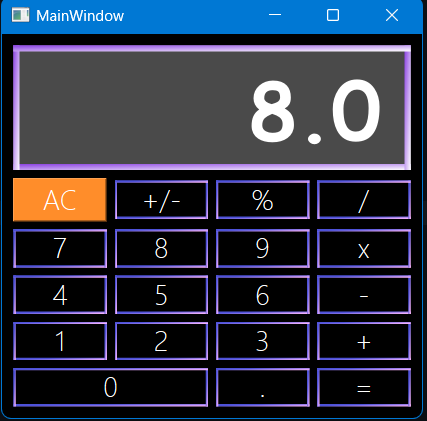
\includegraphics[width=\textwidth]{10.png}
    \caption{}
    \label{fig:imagen2}
  \end{minipage}
\end{figure}

\begin{figure}[htbp]
  \begin{minipage}[b]{0.5\textwidth}
    \centering
    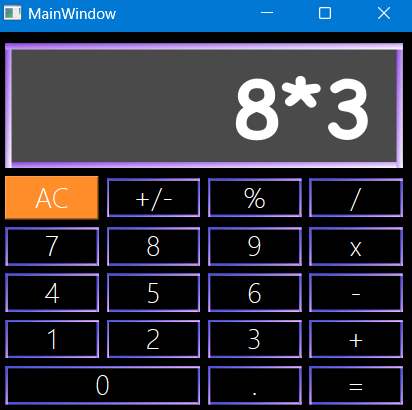
\includegraphics[width=\textwidth]{11.png}
    \caption{}
    \label{fig:imagen1}
  \end{minipage}
  \hfill
  \begin{minipage}[b]{0.5\textwidth}
    \centering
    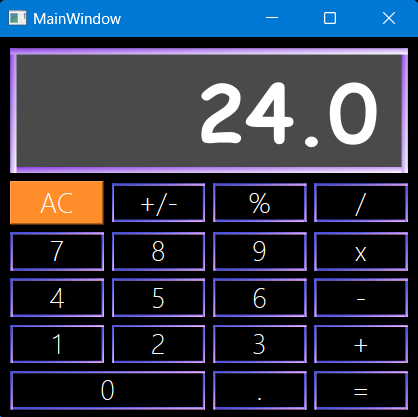
\includegraphics[width=\textwidth]{12.png}
    \caption{}
    \label{fig:imagen2}
  \end{minipage}
\end{figure}

\begin{figure}[htbp]
  \begin{minipage}[b]{0.5\textwidth}
    \centering
    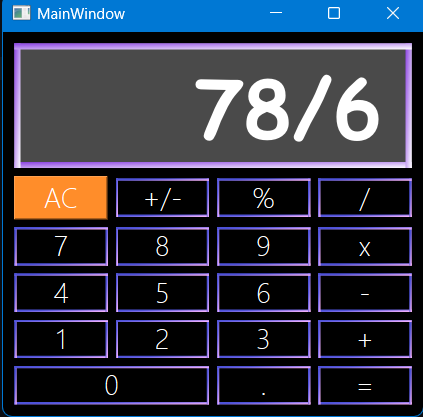
\includegraphics[width=\textwidth]{13.png}
    \caption{}
    \label{fig:imagen1}
  \end{minipage}
  \hfill
  \begin{minipage}[b]{0.5\textwidth}
    \centering
    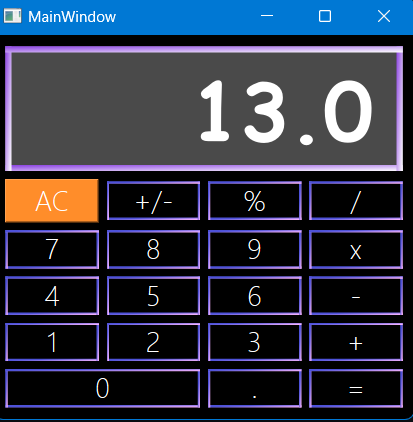
\includegraphics[width=\textwidth]{14.png}
    \caption{}
    \label{fig:imagen2}
  \end{minipage}
\end{figure}

\newpage
\section{Conclusiones.}
Esta practica fue un gran reto para mi, considerando que debemos tener claro los conceptos de programacion orientada a objetos, cuyos ejercios estuvimos trabajando en practicas pasadas, donde estas practicas me sirviero para poder comprender la implementacion de los metodos para poder lograr el funcionamiento de la calculadora,cabe mencionar que la idea es similar a las interfaces de matlab, las cuales tengo un poco mas de experiencia manejando, pero no dejando de lado la importancia de este lenjuagje para futuros poyectos

%%%%%%% Bibliografía %%%%%%%%    

%\appendix  
%\clearpage % o \cleardoublepage
%\addappheadtotoc 
%\appendixpage

%\section{Anexos 1.}




%\section{Anexos 2.}


 

\end{document}
